Darbe kurtas rekurentinis neuroninis tinklas buvo realizuotas C++ programavimo kalba. Naudojama operacinė sistema yra Ubuntu, kuri yra sukurta Linux pagrindu. Projektas buvo saugomas gitHub repozitorijoje.
\clearpage

\begin{figure}[h!]
  \centering
\scalebox{0.45}{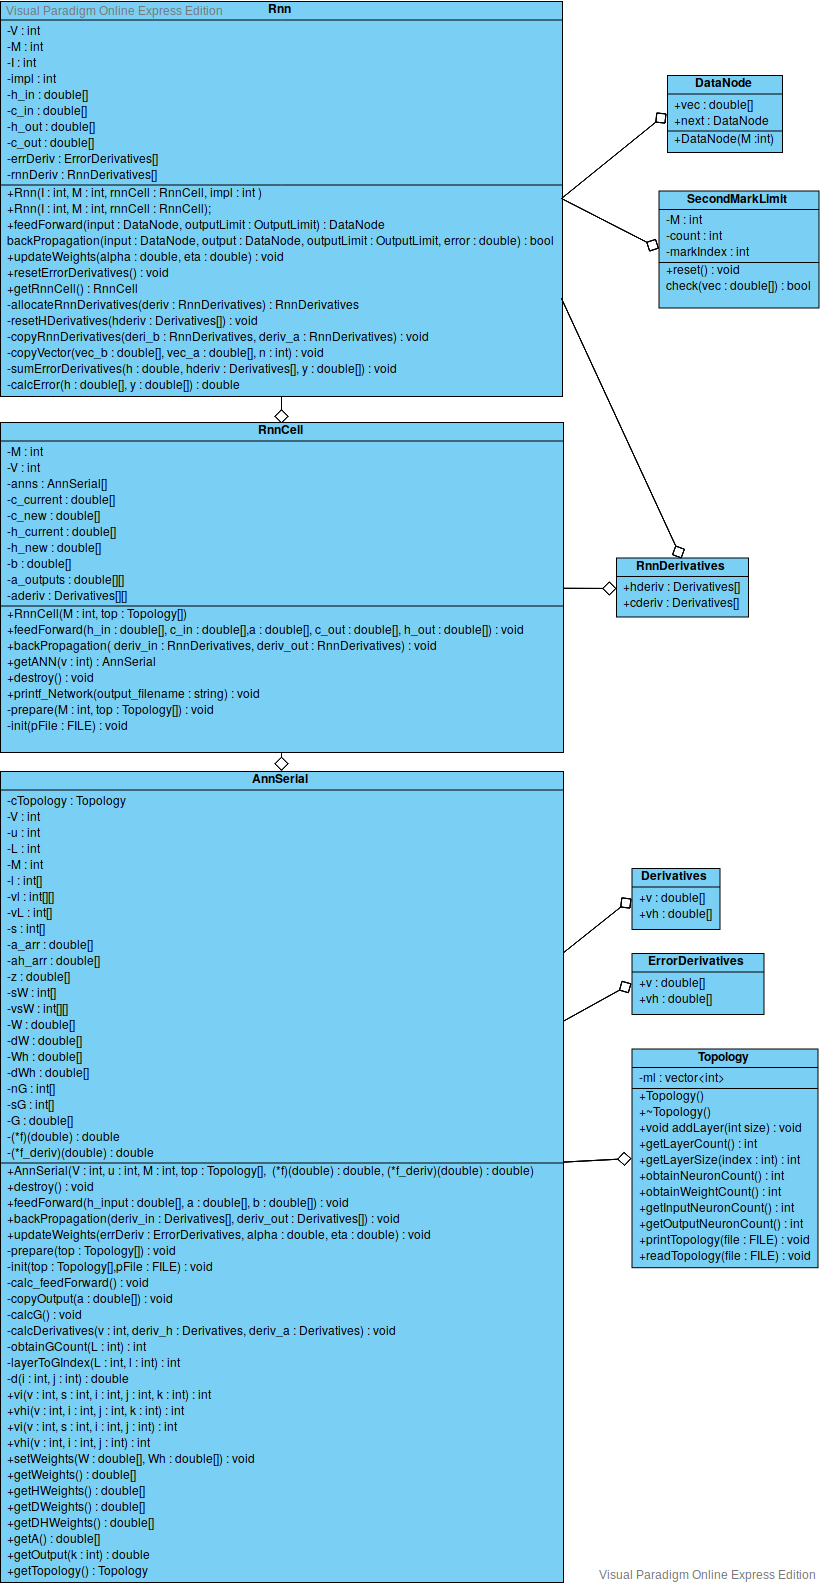
\includegraphics[trim=0 0 0 0cm, clip]{images/new_diag2.png}}
\caption{Klasiu diagrama}
\label{fig:classdiag}
\end{figure}

\clearpage
Tinklui realizuoti buvo sukurtos klasės, kurios aprašo tinklo veikimą.

\begin{enumerate}
  \item \textbf{Rnn} - klasė, kuri kontroliuoja viso tinklo veikimą. Apdoroja įvesties duomenis, apskaičiuoja prognozuojamas reikšmes, tinklą apmokina.
  \item \textbf{RnnCell} - klasė, kuri kontroliuoja rekurentinio neuroninio tinklo skaičiavimus susijusius su viena apmokymo ar prognozavimo iteracija.
  \item \textbf{AnnSerial} - klasė, kuri kontroliuoja paprastų neuroninų tinklų skaičiavimus susijusius su viena apmokymo ar prognozavimo iteracija.
  \item \textbf{Topology} - klasė, kuri saugo atitinkamo neuroninio tinklo struktūrą.
  \item \textbf{Derivatives} - klasė. kuri saugo atitinkamo tinklo išvesčių išvestines, pagal atitinkamo neuroninio tinklo svorius.
  \item \textbf{ErrorDerivatives} - klasė. kuri saugo viso tinklo išvesčių išvestines, pagal atitinkamo neuroninio tinklo svorius.
  \item \textbf{RnnDerivatives} - klasė, kuri saugo visų tinklų išvestines, pagal visų tinklų svorius.
  \item \textbf{SecondMarkLimit} - klasė, kuri skaičiuoja kiek kartų atitinkamas simbolis buvo panaudotas, pagal kurį yra prognozuojamas tekstas.
\end{enumerate}

\clearpage

\begin{figure}[h!]
  \centering
\scalebox{0.8}{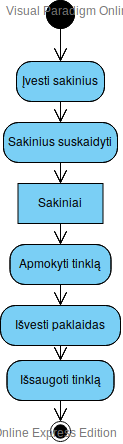
\includegraphics[trim=0 0 0 0cm, clip]{images/Drawing0.png}}
\caption{Veiklos diagrama.}
\label{fig:activity}
\end{figure}

\ref{fig:activity} paveiksle pavaizduota tinklo apmokymo veiklos diagrama. Iš pradžių yra paduodami duomenys į tinklą, šie duomenys yra suskaidomi į sąkinius. Tinklas apmokomas tinklą apmokinant kas vieną sakinį ir grąžinant to sakinio apmokymo vidutinės paklaidos reikymę. Kai yra apmokomi visi sakiniai tinklas gražina kiek laiko mokinosi ir išsisaugo apmokinto tinklo parametrus, kad jį būtų galima naudoti ateityje prognozuojant reikšmes.
